%!TEX root = /Users/domaubert/Documents/Lectures/cosmologie/cosmo_main.tex

\chapter{Histoire thermique de l'Univers et Nucléosynthèse primordiale}

Dans ce chapitre nous allons voir comment les processus à l'œuvre dans l'Univers chaud vont conduire aux abondances observées actuellement des principales particules élémentaires et des éléments légers. Ces processus se déroulent pour $t<3$ minutes, dans un Univers dont la dynamique est dominée par les espèces relativistes. On rappelle que la température décroit avec le temps, tout comme les énergies $k_B T$ caractéristiques associées \sidenote{on rappelle que le $MeV$ désigne 1 million d'électrons-volts constitue une énergie équivalente à $1 MeV \sim 1.6 \times 10^{13} J$} :
\begin{equation}
T\approx\frac{10^{10} K}{\sqrt{t\mathrm{(sec)}}} \approx \frac{1}{k_B}\frac{1 \mathrm{MeV}}{\sqrt{t\mathrm{(sec)}}}.
\end{equation}
On note que ces températures varient en $1/\sqrt{t}$, reflétant ainsi la dépendance en $1/a$ de la température du CMB et le comportement en $a\sim \sqrt{t}$ du facteur d'expansion dans les époques dominées par le rayonnement.
 
\section{Quelques étapes}
On rappelle que 2 processus sont en compétition: l'annihilation\index{annihilation} qui tend à faire décroître de façon exponentielle l'abondance d'une particule donnée et le gel \index{gel des réactions}qui tend à figer l'abondance de cette particule en la soustrayant au bain de réactions environnant. La séquence suivante donne un aperçu de la cascade de processus qui opèrent lors de la baisse de température de l'Univers\index{température}, induite par l'expansion, $T=T_0(1+z)$ \sidenote{Cette température est celle du rayonnement de fond diffus avec $T_0\sim 2.73$ K}. La séquence suivante démarre au confinement des quarks\index{quarks} dans les nucléons.
\newline
\begin{itemize}
\item $T\sim 3\cdot 10^{12}$ K : ($t\sim 10^{-5}$ sec , $kT \sim 250$ MeV) : confinement des quarks. Particules présentes $p,n, \pi^+,\pi^0, \pi^-, e,\bar e, \mu \bar \mu$ + neutrinos\index{neutrinos} ($\nu_e,\bar \nu_e, \nu_\mu, \bar \nu_\mu$).\\
Les particules $\tau, \bar \tau$ sont déjà annihilées à ce stade et les neutrinos associés $\nu_\tau, \bar \nu_\tau$ sont gelés.
 \item $T\sim 10^{12}$ K : désintégration des pions\index{pions}
 \item $T\sim 10^{11}$ K : désintégration des muons\index{muons} et gel des neutrinos associés
 \item $T\sim 6 \cdot 10^{9}$ K : ($kT \sim 500$ keV, t$\sim 1$ s) désintégrations des électrons\index{electrons@électrons}. Gel des $\nu_e$ et gel des abondances relatives de $n$ et $p$.
 \item $T\sim 10^9$ K : démarrage de la nucléosynthèse\index{nucléosynthèse}
 \item $T\sim 3000$ K : recombinaison\index{recombinaison}, production du fond diffus\index{fond diffus}
\end{itemize}

\paragraph{Entropie et fond neutrino} 
Parmi les étapes mentionnées précédemment on constate que les neutrinos\index{neutrinos} se découplent de la 'soupe cosmique' en des époques très reculées et toujours dans leur régime relativiste. Comme expliqué au chapitre précédent, le découplage se met en place lorsque le taux d'expansion, codé par le paramètre de Hubble $H=\dot a /a$, devient plus important que le taux de réaction de l'interaction $\Gamma$ que l'on cherche à étudier. Dans ces époques dominées par le rayonnement, le paramètre de Hubble est donné par:
\begin{equation}
H^2\sim H_0^2 \frac{\Omega_r}{a^4}.
\end{equation}
Durant ces époques dominées par le rayonnement le facteur d'expansion croît comme l'inverse de la température, $a\sim 1/T$ et le taux d'expansion varie en :
\begin{equation}
H\sim H_0 T^2 \sqrt{\Omega_r}
\end{equation}
avec $H_0\sim 70 km/s/Mpc$ et $\Omega_r \sim 10^{-4}$. Par ailleurs les neutrinos interagissent avec les électrons en accord avec les processus d'interaction faible dont le taux d'interaction \sidenote{défini par le produit de la section efficace $\sigma$ et de la vitesse typique de rencontre des particules $v$ pour conduire à un volume d'interaction par seconde} typique varie comme :
\begin{equation}
\sigma v \sim G_F^2 E^2 \sim G_F^2 T^2
\end{equation}
où $G_F$ désigne la constante de Fermi. Comme la densité d'une espèce relativiste varie comme $T^3$, le taux de réaction impliquant les neutrinos varie très rapidement avec la température, et décroit plus rapidement que le taux d'expansion au cours du temps \sidenote{on rappelle que la température décroit avec le temps}:
\begin{equation}
\Gamma =n_\nu \sigma v \sim G_F^2 T^5.
\end{equation}
Il arrive donc un instant où les neutrinos se découplent des électrons, donné numériquement par :
\begin{equation}
T\sim 1 \mathrm{MeV}
\end{equation}
donc dans un Univers âgé environ $t=1$ sec .

Par conséquent, lors du passage des électrons dans le régime non relativiste (qui opère plus tard pour $T\sim 511 \mathrm{keV}$), ces même neutrinos ne peuvent donc servir de canaux de désintégration car ils n'interagissent plus avec ceux-ci via l'interaction faible. Cette désintégration se fait donc uniquement suivant:
\begin{equation}
e^-+e^+\rightarrow \gamma
\end{equation}
Ce processus opère à entropie constante\index{entropie}, donc l'entropie des électrons est reversée sur les photons et non vers le neutrinos. On peut montrer que la densité d'entropie de bosons et fermions sont reliées par:
\begin{equation}
s_F=\frac{7}{8}\frac{g_F}{g_B} s_B
\end{equation}
Par conséquent la nouvelle entropie des photons, post-annihilation des électrons est :
\begin{equation}
s'_\gamma=s_\gamma+s_{e+}+s_{e-}=\frac{11}{4}s_\gamma.
\end{equation}
De plus l'entropie d'une espèce relativiste est une fonction directe du cube de sa température : en effet l'entropie varie comme le nombre de particules, $n\sim T^3$ comme vu précédemment \sidenote{alternativement on a l'entropie qui est le rapport de l'énergie interne sur la température $S\sim \frac{U}{T}$ avec $U\sim T^4$ pour un corps noir par exemple.}. Donc nous avons d'une part une espèce relativiste qui aura évolué de façon passive  (les neutrinos avec $s'_\nu=s_\nu$) et une autre qui aura augmenté grâce aux électrons. Donc en fin de désintégration :
\begin{equation}
s'_\gamma=\frac{11}{4} s_\nu
\end{equation}
ou bien
\begin{equation}
T_\nu=\left(\frac{4}{11}\right)^{1/3} T_\gamma
\end{equation}
Le gaz de neutrino doit être plus froid que celui de photons. Le fond neutrino peut en principe être mesuré aujourd'hui (même si cela reste encore pratiquement impossible) et doit donc présenter une température de  $T_{\nu,0}=1.95 K$\index{température!neutrinos}.

\section{Synthèse de l'hélium}
La synthèse de l'hélium\index{hélium} constitue l'évènement majeur de la production des éléments légers lors de la phase chaude du Big-Bang. L'abondance finale de cet élément va essentiellement dépendre du matériau à disposition et donc de la quantité de nucléons disponible.

\paragraph{Rapport neutron/proton}
 Environ 1 seconde après le Big-Bang, les nucléons (protons et neutrons) ne sont plus relativistes et leurs abondances (notées $p$ et $n$ respectivement pour les protons et neutrons) sont régies par une statistique de type Maxwell-Boltzmann\index{Maxwell-Boltzmann}
\begin{equation}
p\approx n \sim e^{-\frac{m_p c^2}{k_B T}}.
\end{equation}
Les abondances des deux nucléons suivent des évolutions similaires car leurs masses sont proches : le proton\index{proton} est constitué du triplet de quarks\index{quarks} $uud$  et possède une masse de $m_p=938.27$ MeV, tandis que le neutron\index{neutron} est composé du triplet $udd$, pour une masse $m_n=939.56$ MeV. En toute rigueur néanmoins, l'écart de masse $\Delta m=m_n-m_p=1.3$ MeV suffit pour favoriser l'abondance du proton par rapport à celle du neutron, dont l'évolution en abondance est plus rapide. Le rapport d'abondance est donné par:
\begin{equation}
\frac{n}{p}=e^{-\frac{\Delta m}{k_B T}},
\end{equation}
Le gel des réactions impliquant neutrons et protons se produit environ 2 secondes après le Big-Bang. A cet instant le rapport neutrons sur protons vaut:
\begin{equation}
\left(\frac{n}{p}\right)_\mathrm{gel}\approx\frac{1}{6}.
\end{equation}

\paragraph{Synthèse du Deutérium}
Le Deutérium\index{Deutérium} est un noyau composé d'un proton et d'un neutron \sidenote{c'est un isotope de l'hydrogène à partir duquel est fabriquée l'eau lourde $D_2O$ par exemple} et il fait office d'étape intermédiaire vers la production d'hélium. La production de cet élément se fait via la réaction:
\begin{equation}
p+n\leftrightarrow D+\gamma ,
\label{e:deut}
\end{equation}
cette équation doit satisfaire l'équilibre des potentiels chimiques:
\begin{equation}
\mu_p +\mu_n =\mu_D (+0).
\end{equation}
A partir de l'équation \ref{e:nonrel}, ces potentiels chimiques peuvent être extraits pour chaque espèce. En appliquant alors l'égalité des potentiels on obtient l'équation de Saha\index{equation@équation de Saha}
\begin{equation}
X_D=n \times \frac{g_D}{g_n g_p} \left(\frac{2\pi \hbar^2}{kT}\right)^{3/2}\left(\frac{m_D}{m_n m_p}\right)^{3/2} \times e^{\frac{B}{kT}},
\end{equation}
où $X_D=\frac{n_D}{p}$ est le rapport deutérium sur proton et $B=2.22$ MeV est l'énergie de liaison de l'élément\index{energie@énergie de liaison}. Il est d'usage d'exprimer l'abondance de neutrons $n$ en fonction de l'abondance de photons $n\sim \eta n_\gamma$:
\begin{equation}
n\approx 0.244 \eta \left(\frac{k_BT}{\hbar c}\right)^3.
\end{equation}
La dépendance globale de l'abondance du deutérium peut alors se résumer à:
\begin{equation}
X_D\sim(k_BT)^{3/2}\eta e^{\frac{B}{k_B T}}.
\label{e:saha}
\end{equation}
Il apparaît une énergie caractéristique donnée par l'énergie de liaison $B\approx 2$ MeV~: à première vue, en se plaçant quelques secondes après le Big-Bang, la température a suffisamment baissé pour pour que le deutérium devienne suffisamment abondant, via le terme exponentiel de l'équation de Saha. Toutefois les réactifs sont peu abondants ou à l'inverse les photons sont extrêmement nombreux et empêche un déplacement significatif de l'équation \ref{e:deut} vers la production de deutérium : dans l'équation \ref{e:saha} cela se manifeste par le terme $\eta \ll 1$ qui amortit le terme exponentiel. Il faut donc attendre une évolution significative de la température pour que in fine le deutérium puisse être produit en quantité abondante. Ce blocage au niveau du deutérium au cours de la chaîne de synthèse de l'hélium constitue un goulot d'étranglement\index{Deutérium!bottleneck} on parle de \textit{deutérium bottleneck}.

\paragraph{radioactivité $\beta$} En pratique il faut attendre environ 100 secondes, au bout duquel $k_B T\sim 0.1$ MeV pour que l'abondance de deutérium soit suffisante pour poursuivre la synthèse des éléments légers. Pendant ce délai, le rapport $n/p$ continue de décroît sous l'effet de la radioactivité $\beta$ \index{radioactivité} qui conduit à la transformation de neutrons en protons via l'émission d'électrons. La durée de vie du neutron étant de l'ordre de 15 minutes, la modification du rapport est faible mais réelle. A la fin du deutérium bottleneck, nous avons:
\begin{equation}
\left(\frac{n}{p}\right)_\mathrm{bottleneck} \sim \frac{1}{7}
\end{equation}

\paragraph{synthèse de l'hélium et autres éléments légers}
Le deutérium devenant disponible, l'hélium peut être synthétisé. L'énergie de liaison de ce noyau est très importante $B_{He}\sim 30$ MeV, la synthèse est quasi immédiate et quasi totale quand les températures typiques sont de l'ordre de $k_B T < 0.1$ MeV : l'intégralité des neutrons se trouvent piégés dans les noyaux d'hélium (2 protons + 2 neutrons). Disposant à cet instant de 7 protons pour chaque neutrons, cela conduit à une fraction de masse sous forme d'hélium\index{hélium!fraction de masse} donnée par
\begin{equation}
Y_\mathrm{He}\sim 25\%
\end{equation}
En nombre, l'hélium représente seulement $10\%$ des noyaux, le reste étant quasi-exclusivement des protons, i.e. des noyaux d'hydrogène.

\begin{figure}[htbp]
	\centering
		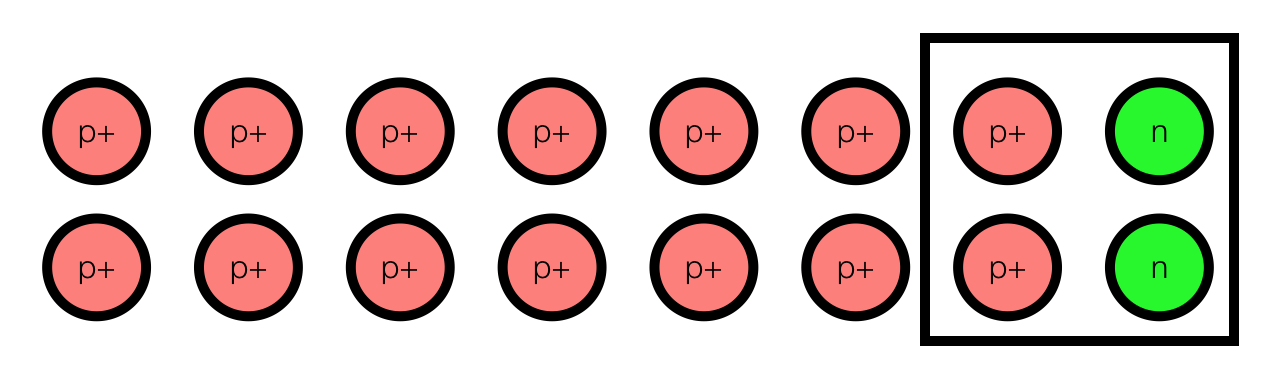
\includegraphics[height=12cm]{figs/helium.png}
	\caption[La situation après la fin du goulot du Deutérium]{La situation après la fin du goulot du 'Deutérium'. Chaque groupe de 8 nucléons contient environ 1 neutron : un noyau d'hélium peut donc être fabriqué pour 16 nucléons, donnant un rapport de masse final d'environ 25\%.}
	\label{f:helium}
\end{figure}

Quelques éléments supplémentaires sont également produits. Par exemple le Li$^7$\index{lithium} est un élément produit en faible quantité à partir de l'hélium, ainsi que He$^3$ qui est un résidu des réaction de production de He$^4$. D'autres éléments comme Be$^7$ \index{béryllium} et H$^3$ sont également synthétisés mais leur temps de vie courts par rapport à l'âge de l'Univers font que ces éléments ne sont plus présent aujourd'hui. 

De façon générale c'est la grande stabilité du noyau d'hélium standard qui lui confère ce rôle prédominant. La Figure \ref{f:binding} présente une mesure de la stabilité des différents éléments en fonction de leur masse. Dans ce diagramme on constate que l'élément le plus stable de la nature est le Fer. Si l'on part des éléments les plus lourds (tels l'Uranium) et que l'on réalise de la fission nucléaire pour fabriquer des éléments plus légers (en se déplaçant vers la gauche dans ce diagramme), des éléments plus stables sont crées produisant ainsi de l'énergie. De même si l'on part des éléments les plus légers (tels l'hydrogène) et que l'on en fabrique de plus lourds, on gagne en stabilité et donc on produit de l'énergie : c'est le principe de fusion nucléaire. Toutefois l'on constate que l'hélium constitue un îlot de stabilité : il n'y a donc pas d'incitation naturelle à produire des éléments plus lourds à partir de celui-ci en fabriquant l'élément plus lourd qui lui succède immédiatement, à savoir le Lithium. Les autres éléments de masse voisine sont beaucoup plus instables (avec des énergies de liaison plus faibles) et sont donc peu enclin à se former. Il est ainsi communément dit que la nucléosynthèse primordiale s'arrête avec He$^4$, 3 minutes (i.e. une grosse centaine de secondes) après le Big-Bang. Les éléments plus lourds ne pourront être produit que via des processus stellaires, notamment via la réaction triple $\alpha$\index{triple-$\alpha$} :  le produit de cette réaction conduit à la création d'un élément à $3\times 4= 12$ nucléons, à savoir le carbone, dont on constate dans la figure \ref{f:binding}, qu'il est le premier élément plus stable que l'hélium. Les conditions thermodynamiques de l'Univers quelques minutes après le Big-Bang ne permettront toutefois pas de synthèse du carbone dans ces premiers instants.

\begin{figure}[htbp]
	\centering
		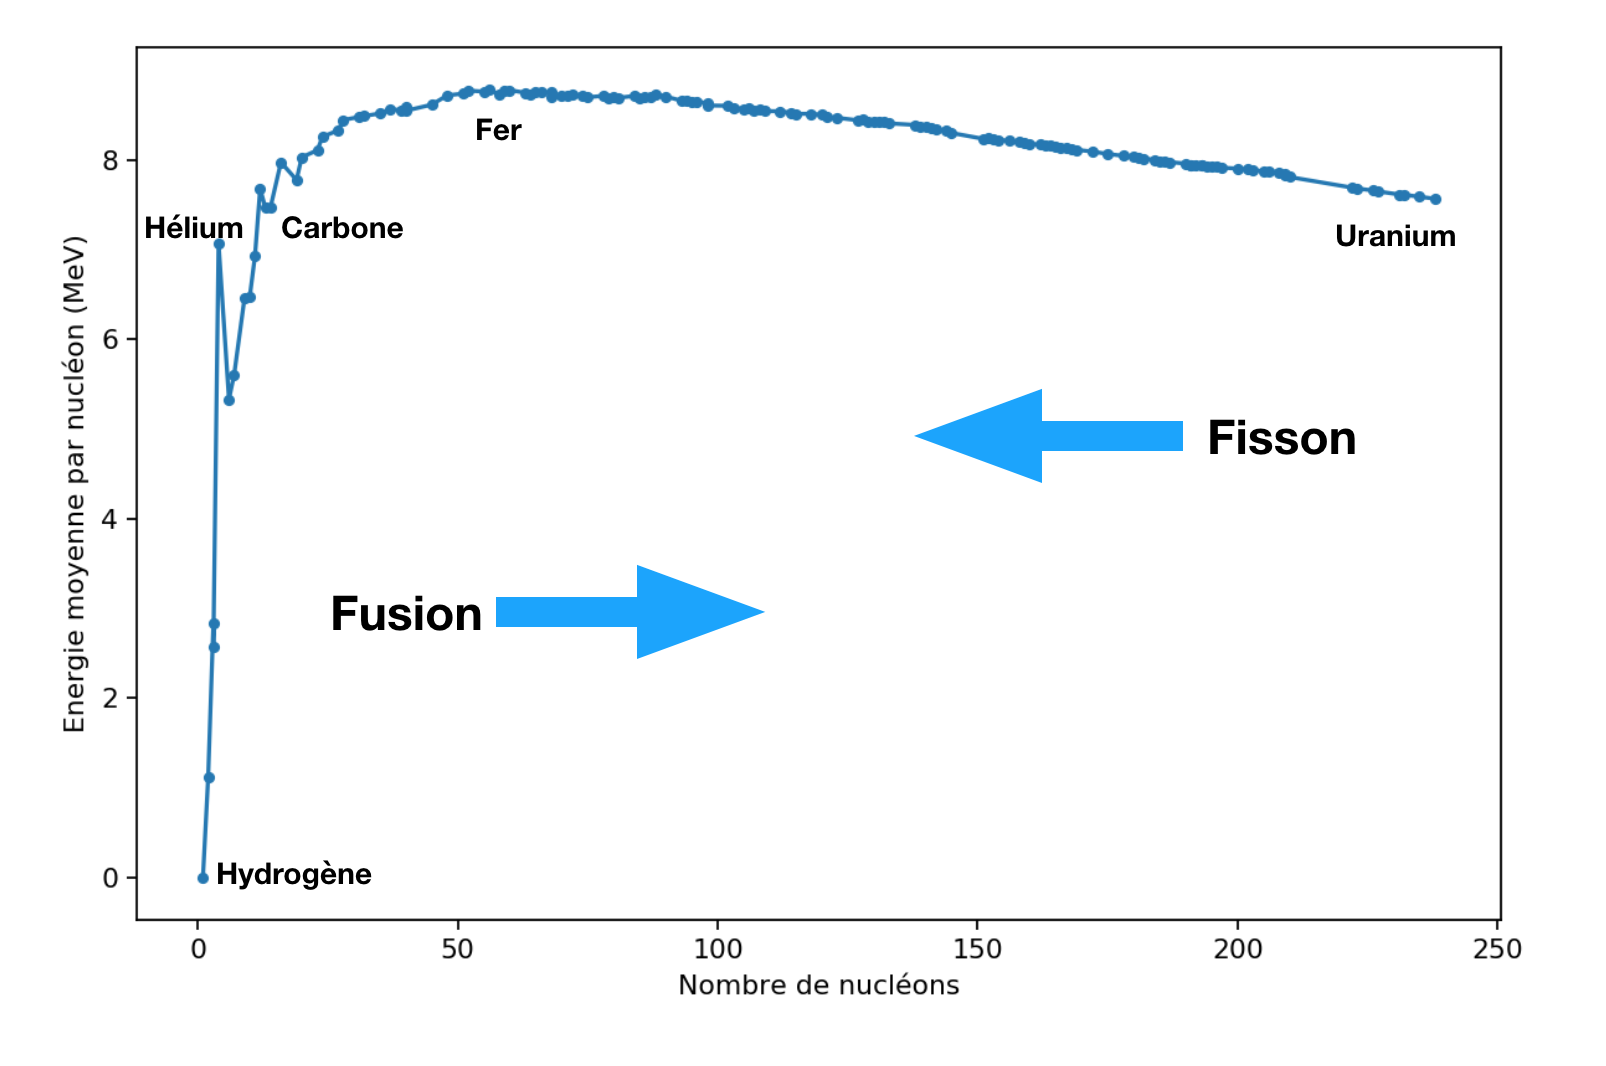
\includegraphics[height=12cm]{figs/binding.png}
	\caption[Energies de liaisons des différents éléments]{L'énergie de liaison moyenne par nucléons des différents éléments et isotopes en fonctions de leur nombre de nucléons. Plus un élément est placé haut dans ce diagramme, plus il est stable. Si l'on fabrique des éléments en se déplaçant vers la droite, on fait de la \textit{fusion nucléaire} et vers la gauche si l'on fait de la \textit{fission}.}
	\label{f:binding}
\end{figure}

\section{Nucléosynthèse et Cosmologie}

La nucléosynthèse primordiale aboutit à la production de quelques éléments légers, dont en particulier l'hélium. Cette production va dépendre du nombre de baryons à disposition, permettant ainsi de contraindre le paramètre $\Omega_b$ ou de façon équivalente le rapport baryons\index{baryons} sur photon $\eta$. La figure \ref{f:nucle} présente la comparaison entre les mesures d'abondances et les modèles de nucléosynthèse primordiale. Les modèles prédisent par exemple que plus l'abondance de baryons est importante, plus la production d'hélium est efficace. En corollaire, l'abondance de deutérium décroit avec la quantité de baryons disponible car précisément cette conversion Deutérium vers hélium se fait plus facilement. Pour le lithium, la situation est plus complexe : dans un premier temps, augmenter le nombre de baryons a tendance à détruire plus facilement cet élément qui est fragile. Dans un second temps, son abondance augmente avec la quantité de baryons car ceux-ci permettent une fabrication plus importante de Hélium-3, He$^3$ et par la suite de Béryllium qui décroit en Lithium. On constate que pour He$^4$ et D, il y a un régime de concordance pour $\eta \sim 6\times 10^{-10}$ et $\Omega_b h^2\sim 0.022$. L'absence d'accord avec le Lithium s'explique quand à lui par la difficulté d'estimer l'abondance \textit{primordiale} de cet élément, cet élément pouvant être détruit au sein des intérieurs stellaires. 

Ces mesures d'abondances issues des théories de nucléosynthèse sont des contraintes très fortes sur la quantité de baryons disponibles : il est aujourd'hui extrêmement difficile de considérer cette quantité comme un paramètre libre. Il est intéressant de constater que ces contraintes sur la quantité de baryons universelle est en accord quasi parfait avec celles issues de l'étude du fond diffus cosmologique (WMAP et Planck)\index{Planck!satellite}. Cet accord est d'autant plus remarquable que ces estimations reposent sur des études très différentes :abondance primordiale d'éléments d'une part, spectre des fluctuations des baryons de l'autre.

Remarquons enfin que les abondances dépendent également de la variation temporelle de la température, régie par l'évolution du facteur d'expansion et donc in fine sur les paramètres cosmologiques. Ainsi les processus de nucléosynthèse se déroule dans une époque où la dynamique de l'Univers est dominée par les espèces relativistes, ainsi dans l'absolu les abondances permettent de contraindre la densité d'énergie des espèce relativistes $\Omega_r$ \index{densité! énergie des espèces relativistes}. Par exemple, le nombre d'espèce de neutrinos\index{neutrinos!nombre} peut être contraint par cette mesure et les résultats actuels ne permettent pas de dévier du nombre de neutrinos prédit par le modèle standard, à savoir 3.


\begin{figure}[htbp]
	\centering
		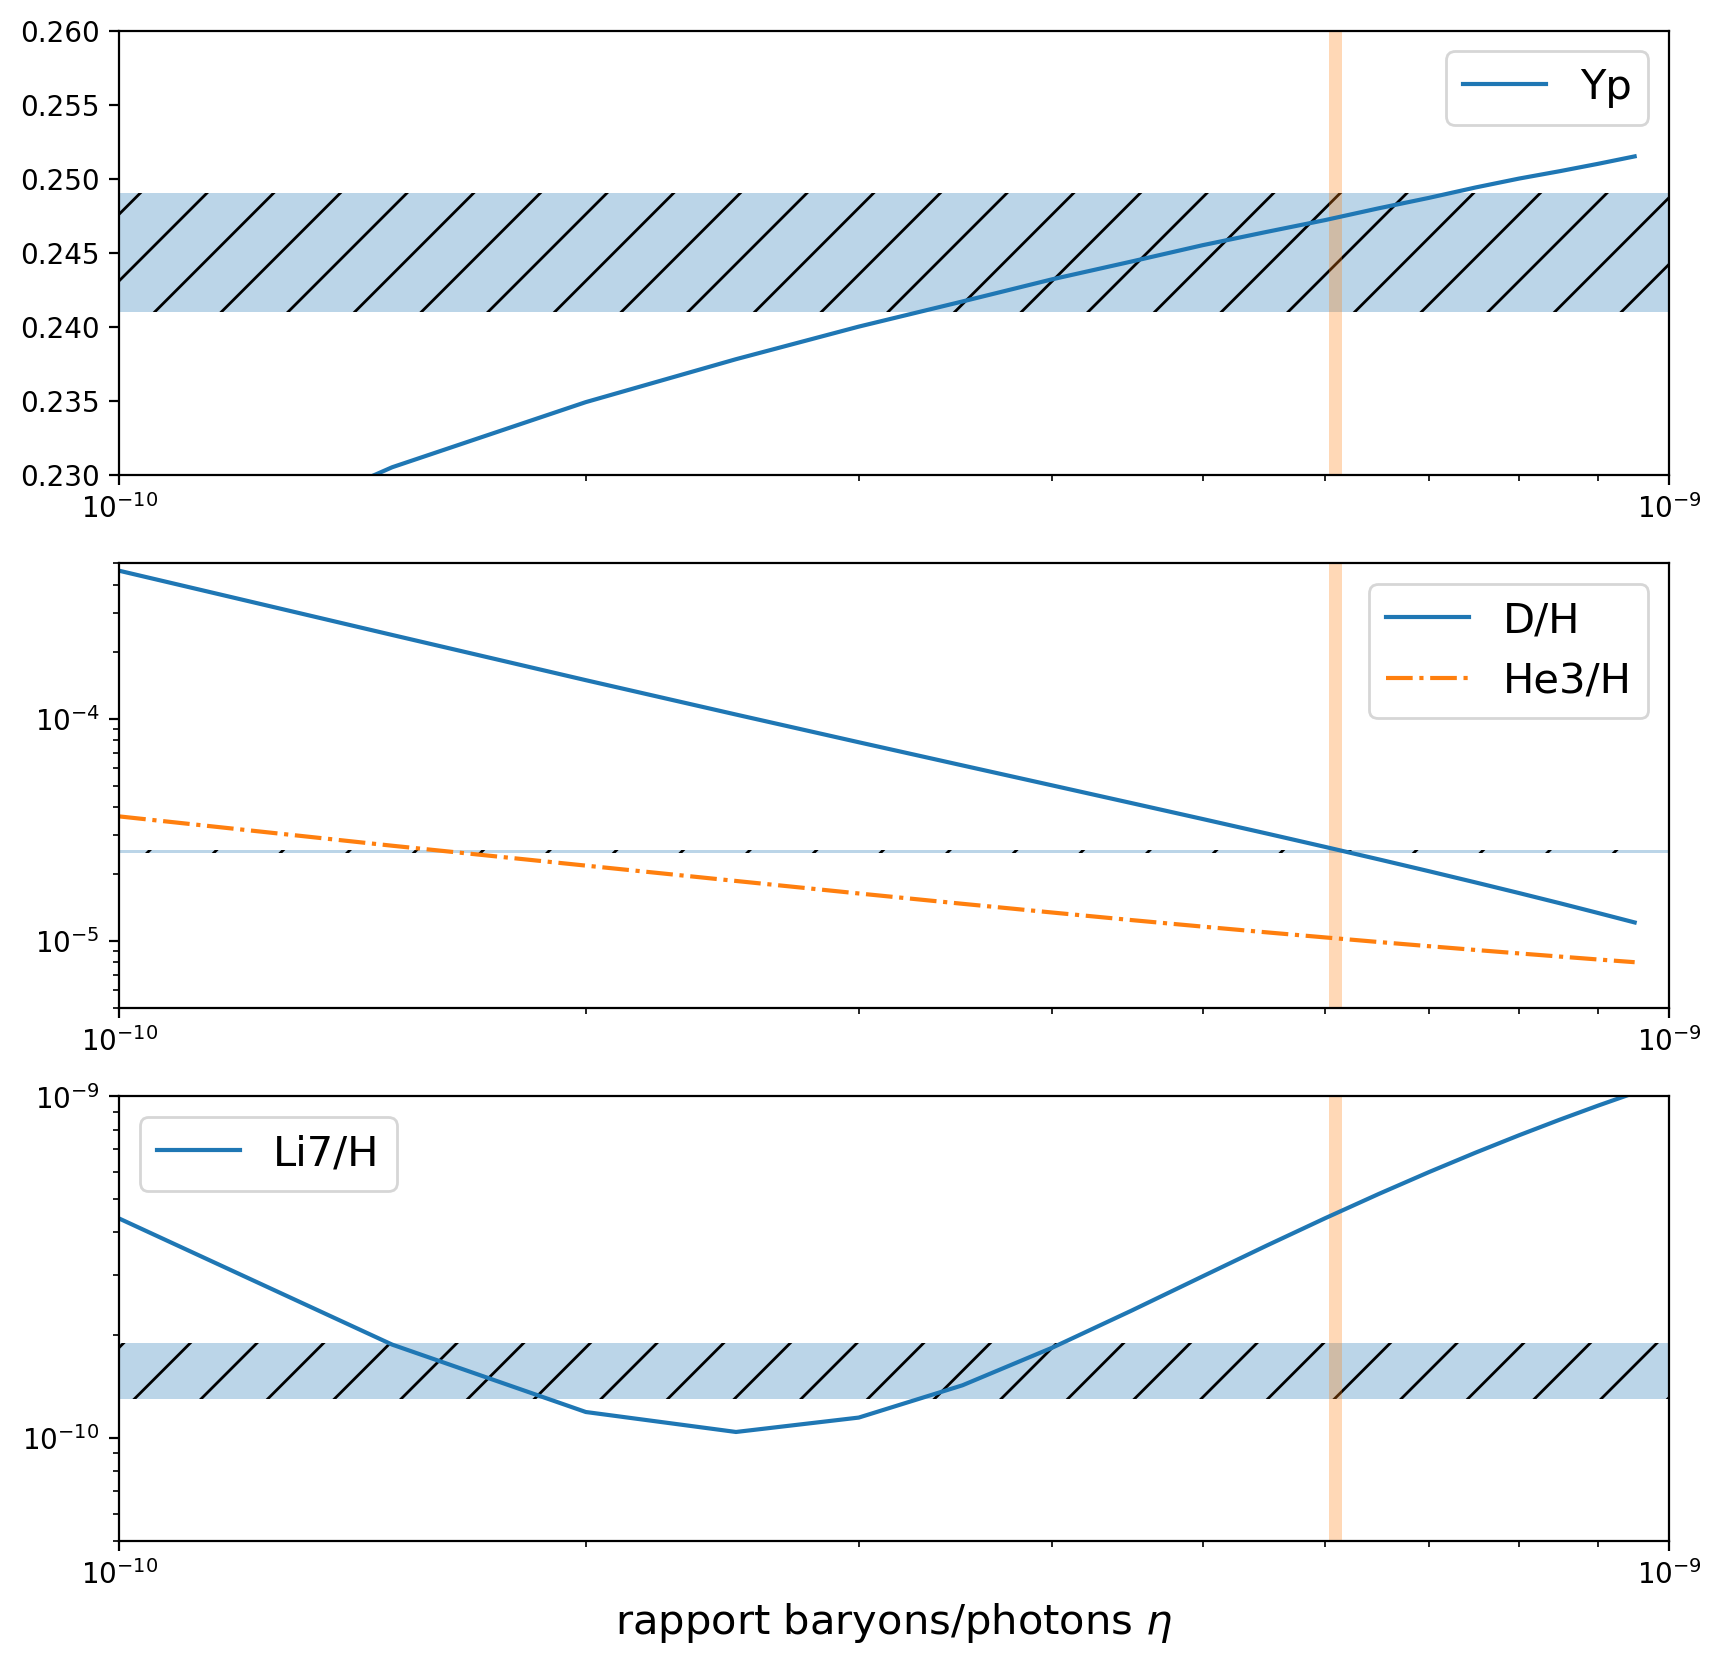
\includegraphics[height=13cm]{figs/BBN.png}
		\caption[Comparaison des abondances observées des éléments légers]{Comparaison des abondances observées des éléments légers (régions bleues horizontales, Fields et al. (2015)), des modèles (lignes) et des contraintes Planck (région orange verticale). Ces abondances sont données en fonction du rapport baryon sur photon  $\eta$. Abondances théoriques calculées avec \textit{AlterBBN} (A. Arbey).}
	\label{f:nucle}
\end{figure}
